During this `embargo period', all researchers with access to the data were under a confidentiality agreement not to discuss the study. This is because the primary researchers wanted to evaluate the predictions of other researchers regarding the study results, and in order to prevent biased/informed opinions, they needed to prevent information leakage between those analyzing the data and those participating in the prediction markets. 

 surveyed the literature to find how many different ways that researchers analyze task-related brain activations using fMRI, and found over 1000 different analysis pipelines. He analyzed the same dataset using all of these pipelines, and found that the results (i.e., peak activations) varied in location across pipelines.
 
 \subsection{Coordinate-based meta-analysis (CBMA}

We are able to perform image-based meta-analyses (IBMAs) because we have the images for each individual analysis team. IBMAs into account more information than coordinate-based meta-analyses. However, it was also of interest.
For the coordinate-based meta-analysis, 





To estimate the proportion of variation related to teams, we compared a) the variance maps across this set of images, to b) variance maps across group-level images from past studies on this topic, gathered from an online repository of result images [BrainMap? NeuroVault? still figuring out if I can get these maps]. Figure [variance maps figure] shows these two variance maps and the difference between the two as an approximation of the effect size 



We will calculate the voxel-wise variance map for this set of group-level images, and compare it to bootstrapped voxel-wise variance maps for sets of group-level activation images from past studies on this topic, using voxel-wise tests of no difference between group maps from this study on the same data and group maps from past studies on different data. 

The data used here is part of the Neuroimaging Analysis Replication and Prediction Study (NARPS, \textit{https://www.narps.info/analysis.html}), and this is not the official report from that larger study. There were nine hypotheses to be tested in this larger study. Here, we examined one hypothesis: that there would be a parametric effect of gain, specifically, a "positive effect in ventromedial PFC - for the equal indifference group" (\url{https://www.narps.info/analysis.html}).




\begin{figure}[!ht]
    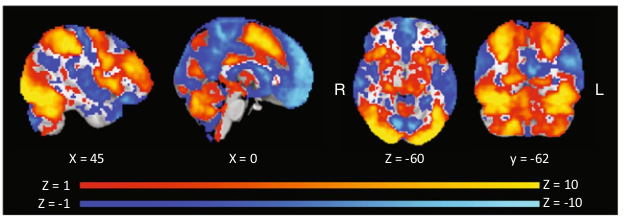
\includegraphics[width=\textwidth]
    {figures/botvinik-nezer_fig4.png}
    \caption{\label{fig:orig_bot} Results from the paper by \cite{botvinik-nezer_fmri_2019}, describing their validation of the original dataset that was used by the analysis teams. Their figure caption is: "Uncorrected results of task versus baseline. Uncorrected Z values are presented, thresholded at Z > 1 for positive activations (hot colors) and Z < −1 for negative activations (cold colors). This analysis was only used for validation." (pp. 7)}
\end{figure}


\begin{figure}[!ht]
    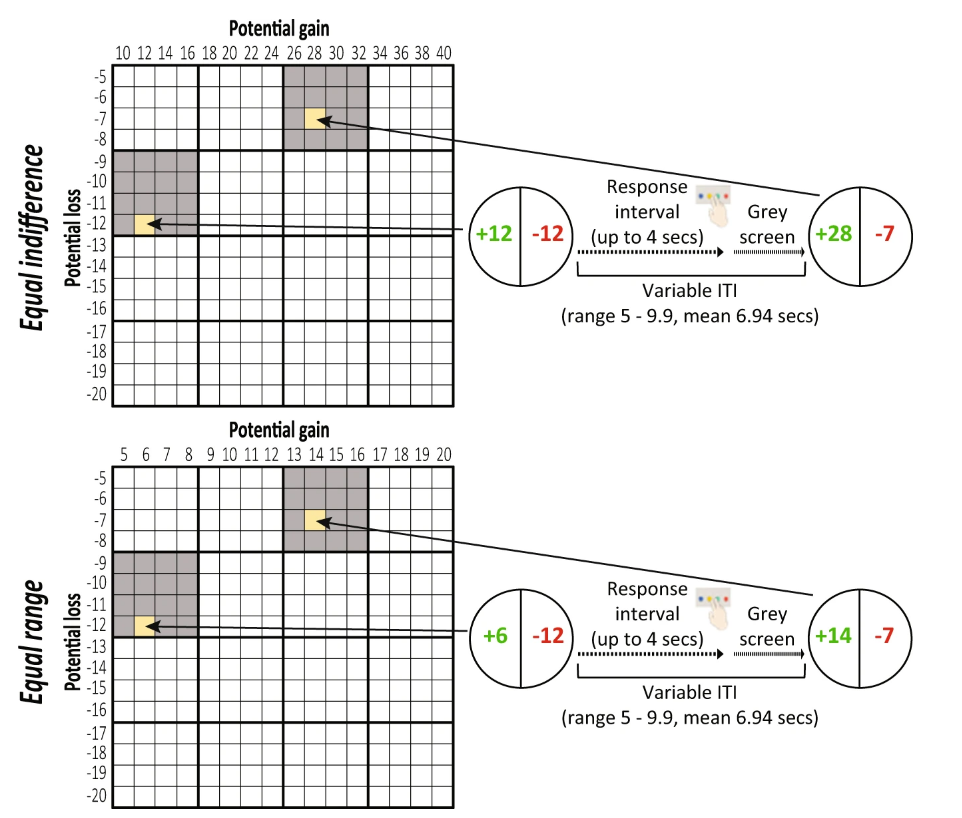
\includegraphics[width=\textwidth]{figures/botvinik-nezer_fig1.png}
    \caption{\label{fig:task} This figure illustrating the behavioral task was taken from \cite{botvinik-nezer_fmri_2019}. This is their caption: ``An illustration of the mixed gambles task design. Adapted from Tom et al.. During each trial, the participant was presented with prospects including the potential gain and loss, until a response was made or four seconds passed. The next gamble was presented following a jittered inter-trial interval (ITI). Potential gains and losses were sampled from the presented gain/loss matrices, which were different for the equal indifference and equal range conditions. The amounts of money are in ILS.''}
\end{figure}






\subsection{Background to the original dataset}
Here we will briefly describe original dataset that was analyzed by the various research teams was fMRI data from participants undergoing the mixed gambles task \citep{tom_neural_2007}. This paradigm is designed to measure decision making in the face of different levels of risk in terms of potential gains and losses. Participants had to decide whether to take a gamble based on the given mixed gamble, that is, the potential gain and potential loss. 

There were two particular paradigms, tested on separate groups of participants. In the 'equal indifference' condition, participants the gains could reach double the losses \citep{tom_neural_2007}; in the 'equal range' condition, the possible ranges of losses and gains were equal \citep{de_martino_amygdala_2010}. Generally, it is thought that people need the gain to be at least twice the potential loss in order to take a gamble (\citealp{tversky1992advances, kahneman1991anomalies, kahneman1990experimental, abdellaoui2007loss}, c.f., \citealp{gal2018loss}); hence the name of the equal indifference condition. See Figure \ref{fig:orig_bot} for the results from the original \textit{Science} paper on this topic. 

The data used here is part of the Neuroimaging Analysis Replication and Prediction Study (NARPS, \textit{https://www.narps.info/analysis.html}). Note that this is not the official report from that larger study; the official report has not been published, and I am not aware of how they are analyzing their data. 

\begin{figure}[!ht]
    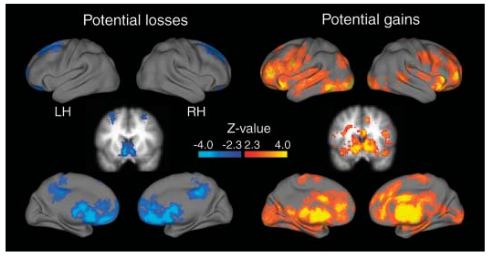
\includegraphics[width=\textwidth]
    {figures/tom_fig2.png}
    \caption{\label{fig:orig_tom} Results from the original paper on this topic by \cite{tom_neural_2007}. Their figure caption is: "Whole-brain analysis of parametric responses to size of potential loss (left) or gain (right). Statistical maps were projected onto an average cortical surface with the use of multifiducial mapping in CARET software \citep{van2005population}; coronal slices (y = 10) are included to show ventral striatal activation. All maps are corrected for multiple comparisons at the whole-brain level by means of cluster-based Gaussian random field correction \citep{worsley1992three} at P < 0.05. LH, left hemisphere; RH, right hemisphere." (pp. 516)}
\end{figure}



 this time carrying the level-2 variance for each team (i.e., SSE\textsubscript{b}, the sum of $\delta_{i}^2$, or the sum of squared errors between participants) into the mixed-effects model. 
 
 
 We can project the original variables into these dimensions multiplying the original matrices of variables with their corresponding singular matrices. In order to find dimensions that are useful for explaining our data, we correlated the projected variables with the original variables using Pearson's correlation. The significance of these 
